%chktex-file 36
%chktex-file 23
%chktex-file 10
%chktex-file 17
%chktex-file 9
%chktex-file 11

\documentclass[ComputationalMathematics.tex]{subfiles}

\begin{document}

%%%%%%%%%%%%%%~~~~~~~~~~~~~~~~~~~~~~~~~~~~~~~~~~~~~~~~%%%%%%%%%%%%%%%
\section{26th of September 2018 --- F. Poloni}
%%%%%%%%%%%%%%~~~~~~~~~~~~~~~~~~~~~~~~~~~~~~~~~~~~~~~~%%%%%%%%%%%%%%%

\subsection{Orthogonality (II)}
In the previous lecture we introduced some sufficent conditions for matrix orthogonality.

\begin{theorem}
  Let $U \in M(n, \R)$ be an orthogonal matrix and let $x \in \R^n$. Then $\norm{Ux} = \norm{x}$.
\end{theorem}

\begin{proof}
  Instead of proving that $\norm{Ux} = \norm{x}$ we will prove $\norm{Ux}^2 = \norm{x}^2$:\\
  
  $$\norm{Ux}^2 = \tr{(Ux)} (Ux) \numeq{(1)} \tr{x} \tr{U} U x = \tr{x} I_n x = \tr{x} x = \norm{x}$$

  where $\numeq{(1)}$ follows from the definition of transpose of a product.
\end{proof}

\textbf{Geometrically} an orthogonal preserve the norm, so a matrix $A$ represents a symmetry or a rotations on vector $x$ and these operations do not alter the size of vectors.

\begin{figure}[H]
    \centering
    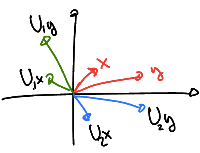
\includegraphics[scale = 0.5]{pics/26sett/orthgonal.png}
\end{figure}

\begin{definition}[Orthogonality]
  Let $x, y \in R^n$ we say that $x$ and $y$ are \textbf{orthonormal} if $\ps{x}{y} = 0$.
\end{definition}

\begin{definition}[Orthonormality]
  Let $x, y \in R^n$ we say that $x$ and $y$ are \textbf{orthonormal} if $\ps{x}{y} = 0$ and $\norm{x} = \norm{y} = 1$.
\end{definition}

\begin{proposition}
  Let us take $U \in M(n, \R)$ such that $U$ is orthogonal. Then its columns $U^1, U^2, \ldots, U^n$ are \textbf{orthonormal} and the same holds for its rows.
  \[
  \tr{U^i} U^j = \begin{cases}
    1 \text{ if } i=j\\
    0 \text{ otherwise}
  \end{cases}
  \]
  and
  \[
    U_i \tr{U_j} = \begin{cases}
    1 \text{ if } i=j\\
    0 \text{ otherwise}
  \end{cases}
  \]
\end{proposition}

\begin{proposition}
  Let $U, V \in M(n, \R)$, such that $U$ and $V$ are orthogonal, then $U V$ is orthogonal. Orthogonal are closed under the product.
\end{proposition}
\begin{proof}
  $\tr{(UV)} (UV) = \tr{V} \tr{U} U V = \tr{V} I_n V = \tr{V} V = I_n$
\end{proof}


\begin{proposition}
We will often deal with tall thin rectangular matrices with
orthonormal columns:
$$ U_1 = [u_1 \; \; u_2 \; \; \dots \; \; u_n] \in \R^{m \times n} \quad (m \geq n)$$

There exists a matrix $U_2$ s.t. $[U_1 \; U_2]$ is square orthogonal.

  
\end{proposition}

\subsection{Eigenvalues / Eigenvector}

\begin{definition}[Eigenvectors and eigenvalues]
  Let $A \in M(n, \R)$ and let $x \neq 0 \in \R^n$ and $\lambda \in \R$.

  If $Ax = \lambda x$ we say that $x$ is an \textbf{eigenvector} of \textbf{eigenvalue} $\lambda$.
\end{definition}

\begin{proposition}
  Let $A \in M(n, \R)$ (real triangular matrix). The eigenvalues of $A$ are the scalars on the diagonal.
\end{proposition}


\noindent \textbf{NOTE}: Eigenvectors and eigenvalues are interesting because we can use it to get a special decomposition of a matrix $A$.\\

\noindent \textbf{Eigendecomposition of a matrix}:\\
For almost almost all matrices $A \in \R^{n \times n}$ under some conditions we can decompose $A$ as:
 $$A = V \Lambda \inv{V}$$
\[
  A = V \Lambda \inv{V} = \begin{pmatrix}
    \\
    v_1 & v_2 & \cdots & v_n\\
    \\
  \end{pmatrix} 
  \begin{pmatrix}
    \lambda_1\\
    &\lambda_2\\
    && \ddots\\
    &&&&&\lambda_n\\
  \end{pmatrix} 
  \begin{pmatrix}
    w_1\\
    w_2\\
    \vdots\\
    w_n\\
  \end{pmatrix}
\]

where $v_i, \; \forall i=1, \ldots, n$ are eigenvectors of $A$ of eigenvalue $\lambda_i$ and $w_i = \text{rows of } V^{-1}$.\\

%% not in 2019
\begin{comment}
This is due to the fact that $\forall B \in R^n$ s.t. $Vx=b$, $x = \begin{pmatrix}
  0\\
  \vdots\\
  0\\
  1\\
  0\\
  \vdots\\
  0
\end{pmatrix}$, where the $1$ is found at position $i$ and so $AV^i=V \Lambda \inv{V} V^i = V \Lambda e_i = \lambda_i V^i$.
\end{comment}
Another way to see the diagonalized form of $A$ is the following:
$$ A = V \Lambda \inv{V} = \sum\limits_{i=1}^{n} v_i\lambda_i w_i^T = $$
$$    \tallthin{$v_1$} \real{$\lambda_1$} \shortlarge{$w_1^T$} + \tallthin{$v_2$} \real{$\lambda_2$} \shortlarge{$w_2^T$} + \cdots + \tallthin{$v_n$} \real{$\lambda_n$} \shortlarge{$w_n^T$}
$$

\syntax{Notice that in Matlab the eigenvalues and eigenvectors of a matrix are computed using the command \texttt{[V, Lambda] = eig(U)} and this operation has a computational complexity of $O(n^3)$.\\ We can check that the matrix \texttt{A} is equal to the decomposition in this way:\\ \texttt{A - V * Lambda * inv(V)} or \texttt{norm(A - V * Lambda * inv(V))} (both should be near to zero).}

Notice that not all matrices $A \in M(n, \R)$ allow a diagonal decomposition.
It may happen that such a matrix is diagonalizable in $\mathds{C}$ and its eigenvalues are complex.

\begin{proposition} If this factorization with eigenvalues and eigenvectors holds, then:
  $$ A = V \Lambda \inv{V} \Longrightarrow Av_i = v_i\lambda \; , \; \forall i = 1, \dots, n $$
\end{proposition}

\noindent This decomposition tell us the behavior under repeated application of a matrix $A$ to a vector $x$. This process allow to scale a general vector $x$.\\

\syntax{
e.g. \texttt{A = [1 1; 1 1]} and \texttt{x = [1 1]}\\
then \texttt{A * x} is equal to \texttt{[2 2]'} and \texttt{A * A * x} is equal to \texttt{[4 4]'}.
}

\begin{comment}


\begin{proposition}
  If $A \in M(n, \R)$ is diagonalizable (aka may be written as $A = V \Lambda \inv{V}$) then $A^k x = \sum\limits_{i=1}^{n} \lambda_i^k \alpha_i V^i$, for some $\alpha_i \in \R$
\end{proposition}

\begin{proof}
  \begin{description}


    \item[{\sc Algebraic view point:}]
      Let us write $x$ in the base of $R^n$ made of the linearly independent columns of $V$:
  \[
x = V^1 \alpha_1 + V^2 \alpha_2 + \cdots + V^n \alpha_n
  \]
  for some $\alpha_i \in \R$.

  \begin{equation}
    \begin{split}
      Ax &= A ( V^1 \alpha_1 + V^2 \alpha_2 + \cdots + V^n \alpha_n)\\
      &= A V^1 \alpha_1 + A V^2 \alpha_2 + \cdots + A V^n \alpha_n\\
      & = \lambda_1 V^1 \alpha_1 + \lambda_2 V^2 \alpha_2 + \cdots + \lambda_n V^n \alpha_n\\
      &= V^1 (\lambda_1 \alpha_1) + V^2 (\lambda_2 \alpha_2) + \cdots + V^n (\lambda_n \alpha_n)\\
    \end{split}
  \end{equation}

  Then
 \begin{equation}
    \begin{split}
      A^2 x &= A \Big (V^1 (\lambda_1 \alpha_1) + V^2 (\lambda_2 \alpha_2) + \cdots + V^n (\lambda_n \alpha_n) \Big )\\
      &= A V^1 \lambda_1 \alpha_1 + A V^2 \lambda_2 \alpha_2 + \cdots + A V^n \lambda_n \alpha_n\\
      &= {\lambda_1}^2 V^1 \alpha_1 + {\lambda_2}^2 V^2 \alpha_2 + \cdots + A {\lambda_n}^2 V^n \alpha_n\\
    \end{split}
  \end{equation}
Inductively, we have proved the theorem.
  
  \item[{\sc Linear algebra view point:}]
    \begin{equation}
      \begin{split}
        A^k x &= A A \ldots A x\\
        &=V \Lambda \cancel{\inv{V}} \cancel{V} \Lambda \cancel{\inv{V}} \ldots \cancel{V} \Lambda \inv{V} x\\
        &= V \Lambda^k \inv{V} x\\
        &=V \begin{pmatrix}
          {\lambda_1}^k\\
          & {\lambda_2}^k\\
          && \ddots\\
          &&&& {\lambda_n}^k\\
        \end{pmatrix}
        \inv{V} x\\
        &=V \begin{pmatrix}
          {\lambda_1}^k\\
          & {\lambda_2}^k\\
          && \ddots\\
          &&&& {\lambda_n}^k\\
        \end{pmatrix}
        \begin{pmatrix}
          {\alpha_1}\\
          {\alpha_2}\\
          \ddots\\
          {\alpha_n}\\
        \end{pmatrix}
      \end{split}
    \end{equation}

  \end{description}
\end{proof}
\end{comment}

\begin{proposition}
  If $A \in M(n, \R)$ is diagonalizable (aka may be written as $A = V \Lambda \inv{V}$) 
  then:
  $$A^k x = \sum\limits_{i=1}^{n} v_i\lambda^k_i w_i^T$$
\end{proposition}

\begin{proof}~\\
  \begin{description}
  \item[{\sc Linear algebra view point:}]
    \begin{equation}
      \begin{split}
        A^k x &= A A \ldots A x\\
        &=V \Lambda \cancel{\inv{V}} \cancel{V} \Lambda \cancel{\inv{V}} \ldots \cancel{V} \Lambda \inv{V} x\\
        &= V \Lambda^k \inv{V} x\\
        &=V \begin{pmatrix}
          {\lambda_1}^k\\
          & {\lambda_2}^k\\
          && \ddots\\
          &&&& {\lambda_n}^k\\
        \end{pmatrix}
        \inv{V} x
      \end{split}
    \end{equation}

  \end{description}
\end{proof}

\noindent \textbf{NOTE}: if $A$ is not square, $Av$, $\lambda v$ have different sizes and it doesn't make sense to talk about eigenvalues.\\

\noindent \textbf{What can go wrong with eigenvalue decomposition}
\begin{enumerate}
    \item  the eigenvalue decomposition is highly non-unique, we can:
    \begin{itemize}
        \item reorder eigenvalues/vectors;
        \item replace an eigenvector $v_i$ with $2v_i \;,\; −3.5v_i \;,\; \dots$;
        \item for matrices with repeated eigenvalues, even more possibilities:\\
        e.g. $I = VIV^-1$ for every invertible $V$.
    \end{itemize}
    
    \item  some matrices have only complex eigenvalues: e.g. $\begin{pmatrix} 2 & 4\\ -3 & 3\end{pmatrix}$;
    
    \item some matrices have fewer eigenvectors than we want and we can't use eigenvalue decomposition: e.g. $\begin{pmatrix} 1 & 1\\ 0 & 1\end{pmatrix}$.
    
\end{enumerate}

\noindent Now, thanks to the eigenvalue decomposition we can prove the following:

\begin{theorem}
  Let $A \in M(n, \R)$. If $\abs{\lambda_i} < 1 $ for all eigenvalues $\lambda_i$ of $A$  then $\lim\limits_{k \to \infty} A^k x = 0$.
\end{theorem}

\begin{theorem}
  Let $A \in M(n, \R)$. If $\forall \lambda_i$ eigenvalues of $A$ $\abs{\lambda_i} < \abs{\lambda_1}$ then $A^k x \approx V^1 {\lambda_1}^k \alpha_1$.
\end{theorem}

\begin{proposition}
  Let $A \in M(n, \R)$ be a diagonalizable matrix and let:
  \[
    A=V\Lambda \inv{V} = \begin{pmatrix}
    \\
    V^1 & V^2 & \cdots & V^n\\
    \\
  \end{pmatrix} 
  \begin{pmatrix}
    \lambda_1\\
    &\lambda_2\\
    && \ddots\\
    &&&&&\lambda_n\\
  \end{pmatrix}
  \begin{pmatrix}
    w_1\\
    w_2\\
    \vdots\\
    w_n\\
  \end{pmatrix}
\]

  Let us now consider a reordering of $V$'s columns and apply the same permutations to the ``diagonal vector'' of $\Lambda$ such that:
  
\[
    \hat{V} = \begin{pmatrix}
    \\
    V^2 & V^1 & V^3 \cdots & V^n\\
    \\
  \end{pmatrix}
  \hat{\Lambda}= \begin{pmatrix}
    \lambda_2\\
    &\lambda_1\\
    &&\lambda_3\\
    &&& \ddots\\
    &&&&&&\lambda_n\\
  \end{pmatrix}
\]

  A can be diagonalized through such $\hat{V}$ and $\hat{\Lambda}$: $A = V \Lambda \inv{V} = \hat{V} \hat{\Lambda} \inv{\hat{V}}$.
\end{proposition}

Moreover, in the case of repeated eigenvalues.

\begin{proposition}
  Let $A \in M(n, \R)$ a diagonalizable matrix such that $A = V \Lambda \inv{V}$, where $\lambda_1 = \lambda_2$ (without loss of generality). Then $V$ can be replaced by $\widetilde{V} = \begin{pmatrix}
    \\
    \\
    V^1 + V^2 & V^1 - V^2 & V^3 & \cdots & V^n\\
    \\
    \\
  \end{pmatrix}$.
\end{proposition}

\begin{theorem}[Spectral theorem]
  Let $A \in S(n, \R)$ ($A$ is a real symmetric matrix). Then $A$ is diagonalizable $A = U\Lambda U^-1$, where eigenvalues are all real numbers and we can take $U$ orthogonal matrix.
\end{theorem}


\noindent For symmetric matrices, nothing goes wrong: eigenvalues decomposition always exists (Spectral theorem). The matrix will not have complex eigenvalues and not fewer eigenvectors. We can choose an $U$ orthogonal because we said it was possible to reorder eigenvalues/vectors and replace eigenvector $v_i$. \\

\syntax{
If we have an symmetric matrix \texttt{B} and we compute \texttt{[V, D] = eig(B)}, Matlab will always return an orthogonal matrix $V$.
}

\noindent \textbf{Quadratic forms}: for a fixed symmetric matrix $Q = Q^T$, consider $x \in \R^{n}$ and $Q \in \R^{n \times n}$ $f(x) = x^T Qx$ (Geometric idea: paraboloids):\\

Let's see two example in a Geometric point of view:\\
Example 1:
$$ f(\begin{pmatrix} x_1\\ x_2 \end{pmatrix}) = \begin{pmatrix} x_1 & x_2 \end{pmatrix}
\begin{pmatrix} 3 & 2 \\ 2 & 4 \end{pmatrix}\begin{pmatrix} x_1\\ x_2 \end{pmatrix}
$$
\begin{figure}[H]
    \centering
    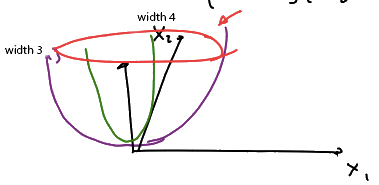
\includegraphics[scale = 0.45]{pics/26sett/quadratic_form_1.png}
\end{figure}

Example 2: 
$$\text{with a matrix } Q = \begin{pmatrix} 3 & 2 \\ 2 & -4 \end{pmatrix}$$
\begin{figure}[H]
    \centering
    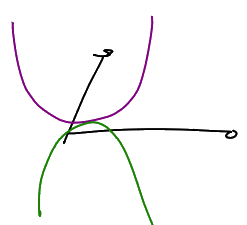
\includegraphics[scale = 0.45]{pics/26sett/quadratic_form_2.png}
\end{figure}

\newpage
\begin{proposition}
  Let $Q \in S(n, \R)$ (For a fixed symmetric matrix) and let $x \in \R^n$. Then:
  $$\lambda_{\text{min}} \sqrnorm{x} \le \tr{x}Qx \le \lambda_{\text{max}} \sqrnorm{x}$$
  where $\lambda_{\text{max}}$ and $\lambda_{\text{min}}$ are respectively the eigenvalue of maximum value and the eigenvalue of minimum value.
\end{proposition}

\begin{proof}~\\
  \begin{description}
    \item[{\sc Easy case with $Q = \Lambda$ diagonal:}]
    
      $$\tr{x}Qx = \tr{x} \begin{pmatrix}
    \lambda_2\\
    &\lambda_1\\
    &&\lambda_3\\
    &&& \ddots\\
    &&&&&&\lambda_n\\
    \end{pmatrix}
    x = \lambda_1 {x_1}^2 + \lambda_2 {x_2}^2 + \cdots + \lambda_n {x_n}^2$$
  It is obvious that this sum is bounded by:
  \[
    \lambda_{\text{min}} ({x_1}^2 +{x_2}^2 + \cdots + {x_n}^2) \le  \lambda_1 {x_1}^2 + \lambda_2 {x_2}^2 + \cdots + \lambda_n {x_n}^2 \le \lambda_{\text{max}} ({x_1}^2 +{x_2}^2 + \cdots + {x_n}^2)
  \]

      The following holds: $ \lambda_{\text{min}} ({x_1}^2 +{x_2}^2 + \cdots + {x_n}^2) =  \lambda_{\text{min}} \tr{x} x =  \lambda_{\text{min}} \sqrnorm{x}$ and, on the other hand, $ \lambda_{\text{max}} ({x_1}^2 +{x_2}^2 + \cdots + {x_n}^2) =  \lambda_{\text{max}} \tr{x} x =  \lambda_{\text{max}} \sqrnorm{x}$ and this proves the fact in the special case of diagonal matrix $Q$.
    \item[{\sc General case:}]
      Let us represent $Q$ through its eigendecomposition: $A = U \Lambda \inv{U} = U \Lambda \tr{U}$, where $U$ is an orthogonal matrix.
      $$\tr{x}Qx = \tr{x} U \Lambda \tr{U} x \numeq{(1)} \tr{y} \Lambda y$$

      where $\numeq{(1)}$ is due to the change of variable $y = \tr{U} x$ (that implies $\tr{y} = \tr{x} U$).

      By the same argument used in the diagonal case:
      $$\lambda_{\text{min}} \sqrnorm{y} \le \tr{y} \Lambda y \le \lambda_{\text{max}} \sqrnorm{y}$$
      Now the point is that if we can replace $\sqrnorm{y}$ with $\sqrnorm{x}$ we have proved the theorem.
      In fact this is true, due to the orthogonality of matrix $U$ ( $UU^T = U^TU = I$.
  \end{description}
\end{proof}

\begin{corollary}
  Let $Q \in S(n, \R)$ and let $x \in \R^n$. If $x \neq 0$, $\lambda_{\text{min}} \le \frac{\tr{x}Qx}{\sqrnorm{x}} \le \lambda_{\text{max}}$, where $\lambda_{\text{max}}$ and $\lambda_{\text{min}}$ are respectively the eigenvalue of maximum value and the eigenvalue of minimum value.
\end{corollary}

\begin{definition}[Positive semidefinite]
  Let $Q \in S(n, \R)$. If $\lambda_i \geq 0$ for each eigenvalue of $Q$ then $\tr{x} Q x \ge 0$ for each vector $x$. $Q$ is called positive semidefinite.
  $$ \tr{x} Q x \ge 0\norm{x}^2 \geq 0$$
  This is Iff, so the reverse holds: if $\tr{x} Q x \ge 0$ for all $x$, then eigenvalues of $Q$ are $\geq 0$.
  \end{definition}

\begin{definition}[Positive definite]
    Let $Q \in S(n, \R)$. If $\lambda_i > 0$ for each eigenvalue of $Q$ then $\tr{x} Q x > 0$ for each vector $x \neq 0$. $Q$ is called positive semidefinite.
    $$ \tr{x} Q x \ge \lambda_{min}\norm{x}^2 > 0\norm{x}^2 = 0$$
    This is Iff, so the reverse holds: if $\tr{x} Q x > 0$ for all $x$, then eigenvalues of $Q$ are $> 0$.

\end{definition}

\begin{proposition}
  Let $Q \in S(n, \R)$. Iff $Q$ is \textbf{positive semidefinite} then $\lambda \ge 0 \; \forall \lambda$ eigenvalue of $Q$ iff $Q$ is \textbf{positive semidefinite}. On the other hand, all eigenvalues are \textbf{strictly} positive iff $Q$ is positive definite.
\end{proposition}

\begin{proof}~\\
Let's prove that iff $Q$ is \textbf{positive semidefinite} then $\lambda \ge 0 \; \forall \lambda$ by contradiction:\\
if $Q$ has a eigenvalue $\lambda_i < 0$ then:
$$ v_i^TQv_i = v_i^T \lambda v_i = \lambda_i\norm{v_i}^2 < 0$$
for the eigenvector $v_i$ associated to $\lambda_i$.
  
\begin{comment}
  %not 2019
  \indent ($\Rightarrow$) $\tr{x} A x \ge \lambda_{\text{min}}$.

  ($\Leftarrow$)Let $v_i$ be an eigenvector of $A$.

  \indent $0 \le \tr{v_i} A v_i = \tr{v_i} ( \lambda_i v_i) = \lambda_i  \tr{v_i} v_i = \lambda_i \sqrnorm{v_i} \Rightarrow \lambda_i \ge 0$.
\end{comment}  
\end{proof}

\begin{proposition}
  Let $B \in M(m, n, \R)$ (possibly rectangular), $\tr{B} B \in S(n, \R)$ is a valid product
and gives a square, symmetric matrix and is positive semidefinite.
\end{proposition}

\begin{proof}~\\
\begin{description}
  \item[{\sc Symmetry:}] $\tr{(\tr{B}B)} = \tr{B} \tr{(\tr{B})} = \tr{B} B$
  \item[{\sc Positive definite:}] $\tr{x} \tr{B} B x = \tr{(B x)} (Bx) = \sqrnorm{Bx} \ge 0$
\end{description}
\end{proof}

\begin{corollary}
The same holds for $B\tr{B}$, since we can define $C = \tr{B}$.
\end{corollary}

\begin{proposition}
  Let $Q \in S(n, \R)$. $A \succeq 0$ and $A$ invertible iff $Q$ is \textbf{strictly positive definite}.
\end{proposition}

\syntax{
  In order to check if a matrix $A$ is positive definite in Matlab we can look at its eigenvalues (cfr. \texttt{eig(A)}).
}

\noindent \textbf{NOTE for complex matrices}:\\
Most of these properties work also for matrices with complex
entries, with one change: replace $A^T$ with $\overline{A^T}$ (transpose +
entrywise conjugate). Often denoted with $A^*$ or $A^H$.\\

\noindent The norm of a complex vector:
$$\norm{x}_2^2 = x^*x = \overline{x_1}x_1 + \overline{x_2}x_2 + \dots + \overline{x_n}x_n = \abs{x_1}^2 + \dots + \abs{x_n}^2 \; \; \text{which is always real} \geq 0$$

\noindent Some terminology changes:
\begin{itemize}
    \item $UU^* = I$: unitary matrix (orthogonal + complex)
    \item $Q = Q^*$: Hermitian matrix (capital letter, after Charles Hermite).
\end{itemize}




\end{document}
